% Requiere graphicx y los PDF de figures/tecplot.


\section{Metodología y alcance}
El estudio utiliza la implementación MATLAB posterior a la revisión energética del 19 de septiembre de 2026. Se mantienen las vigas Timoshenko tridimensionales, la masa consistente, las restricciones exactas raíz--cubo, las propiedades heredadas y la rotación nominal prescrita alrededor del eje 129--130. La velocidad angular $\Omega$ permanece constante en cada evaluación. No se introduce movimiento nominal de guiñada.

Sea $q_0$ el estado de operación y $T_c$ el mapa instantáneo de restricciones. El equilibrio implementado satisface
\begin{equation}
T_c^{\mathsf T}\bigl[f_{\mathrm{ext}}(q_0)-f_{\mathrm{int}}(q_0)\bigr]=0.
\end{equation}
La fuerza interna y su tangente se obtienen de la energía corrotacional de pequeñas deformaciones mediante diferenciación numérica. La masa se conserva en la configuración de referencia. Cada cambio paramétrico exige un nuevo equilibrio, por lo que se calcula sensibilidad total del modelo, incluyendo la variación de la precarga.

Sean $M$, $C$, $G$ y $K_e$ las matrices de masa, amortiguamiento estructural, giroscopía y rigidez elástica. La implementación actual almacena, además, $H_M$ como contribución de transporte denominada \texttt{massRate}, y $K_{\mathrm{tr}}$ como rigidez de transporte. Sea $q$ el vector de perturbaciones físicas. Los operadores del instante de referencia son
\begin{equation}
D=C+G+H_M,\qquad
K=K_e+K_g+K_\Omega+K_a+K_{\mathrm{tr}}.
\end{equation}
Aquí $K_g$ recoge la tangente del equilibrio después de separar la parte elástica y la aerodinámica $K_a$. $K_\Omega$ identifica las contribuciones de giro no incluidas previamente. Se evita duplicar las contribuciones inerciales de orden $\Omega^2$: $K_\Omega=0$ cuando ya están incorporadas en esa tangente. Los términos de orden $\Omega$ y $\Omega^2$ se conservan según la formulación existente.

Para $q=T(t)z$, donde $z$ contiene coordenadas independientes y $T$ incluye el mapa cinemático, se emplean
\begin{align}
M_r&=T^{\mathsf T}MT,\\
D_r&=T^{\mathsf T}(DT+2M\dot T),\\
K_r&=T^{\mathsf T}(KT+D\dot T+M\ddot T).
\end{align}
La transformación homóloga y multiblade conserva también sus derivadas. Los operadores modales resultantes, denotados $M_m,D_m,K_m$, definen el problema cuadrático, con autovalor complejo $\lambda$ y forma modal $\phi$,
\begin{equation}
Q(\lambda)\phi=(\lambda^2M_m+\lambda D_m+K_m)\phi=0.
\end{equation}
Se verifican autovectores derechos e izquierdos; un residuo pequeño no implica por sí solo pequeño error de respuesta \cite{tisseur2001}. Con la convención $\exp(\lambda t)$, se definen crecimiento $\sigma=\operatorname{Re}\lambda$ [$\mathrm{s}^{-1}$], frecuencia amortiguada $f_d=|\operatorname{Im}\lambda|/(2\pi)$ [Hz] y razón de amortiguamiento $\zeta=-\operatorname{Re}\lambda/|\lambda|$ para raíces oscilatorias. El espectro de \texttt{eigs} es parcial. El azimut y los operadores se congelan; no se calcula estabilidad periódica de Floquet.

\subsection{Parámetros, dependencias y respuestas}
Se define el factor $\xi_i=p_i/p_{i0}$, con $p_{i0}$ nominal y $\xi_{i0}=1$. La velocidad nominal es $12$ rpm, equivalente a $1.256637$ rad/s. La tabla~\ref{tab:param} resume los escenarios. Sus intervalos no representan incertidumbre experimental ni distribuciones probabilísticas.

\begin{table}[htbp]
\centering\small
\caption{Factores exploratorios y dependencias conservadas.}\label{tab:param}
\begin{tabular}{>{\raggedright\arraybackslash}p{3.2cm}>{\raggedright\arraybackslash}p{8.4cm}c}
\toprule
Factor & Actualización coherente a geometría fija & Intervalo\\
\midrule
Velocidad del rotor & Equilibrio, giroscopía, transporte, restricciones móviles y MBC & $[0.98,1.02]$\\
Densidad de palas/torre & Masa lineal [kg/m] e inercias seccionales [kg m] vinculadas & $[0.98,1.02]$\\
Densidad de góndola/cubo & Masa [kg] y tensor centroidal completo [kg m$^2$] por cuerpo & $[0.98,1.02]$\\
Rigidez de palas/torre & Seis rigideces proporcionales: EA/GA [N], EI/GJ [N m$^2$] & $[0.98,1.02]$\\
Amortiguamiento & Dos razones Rayleigh de 0.01, con anclas de 0.2 y 2 Hz fijas & $[0.98,1.02]$\\
Rigidez del tren & Matriz relativa ilustrativa, traslación y rotación vinculadas & $[0.98,1.02]$\\
K/C del apoyo & Un factor positivo por matriz del apoyo flexible heredado & $[0.99,1.01]$\\
Amplitud sísmica & Escalamiento común de aceleración, velocidad y desplazamiento del suelo & $[0.99,1.01]$\\
\bottomrule
\end{tabular}
\end{table}

Los símbolos $J_x,J_y,J_z$ designan los momentos seccionales de masa por unidad de longitud en los ejes locales. La masa y todas las inercias de cada familia o cuerpo escalan juntas; se preserva $J_x=J_y+J_z$ en las secciones. No se reconstruyen geometrías de pala, módulos o áreas ausentes. La variación de rigidez es un escenario constitutivo proporcional. Los offsets y productos de inercia son los existentes. Los valores dimensionales y su procedencia se exportan por sección, cuerpo y conexión. La interfaz aerodinámica conserva valor cero por ausencia de datos; no se estudia un modelo aerodinámico inexistente.

Las respuestas incluyen $f_d$, $\sigma$, $\zeta$, centroides de grupos, desplazamientos de equilibrio y máximos sísmicos. Los canales temporales son $u_y$ de maestros 129/130 y $u_z$ de puntas 56/92/128, en ejes globales, con ventana de $0$ a $1$ s. Los máximos de aceleración son absolutos y los de desplazamiento son relativos a la base. La recuperación incluye $\dot T$ y $\ddot T$ de un mismo instante operativo.

\subsection{Diferenciación, seguimiento y aceptación}
Para una respuesta escalar $y$, se calcula
\begin{equation}
d_i(h)=\frac{y(1+h)-y(1-h)}{2h},\qquad
S_i=\frac{d_i(h)}{y_0},
\end{equation}
cuando $y_0$ no es pequeño y no hay cambio de signo. Para $\sigma$ se usa la escala $|\lambda_0|$ [$\mathrm{s}^{-1}$]; para desplazamientos estáticos, $\max(|q_0|,10^{-3}\ \mathrm{m})$. Cada fila registra su normalización. Se comparan $h=0.02,0.01,0.005$ y se exige concordancia de las derivadas consecutivas dentro de $2\,\text{\char37}$, con un piso absoluto documentado en el módulo.

Las formas complejas se comparan en el mismo espacio físico mediante
\begin{equation}
\operatorname{MAC}_{ab}=\frac{|\phi_a^{\mathsf H}M_0\phi_b|^2}
{(\phi_a^{\mathsf H}M_0\phi_a)(\phi_b^{\mathsf H}M_0\phi_b)},
\end{equation}
donde $M_0$ es la masa física nominal y $\mathsf H$ indica transposición conjugada. La asignación global combina MAC y proximidad de raíces complejas. Para grupos próximos se usan ángulos principales y MAC subespacial, evitando interpretar una rotación de la base modal como cambio físico \cite{allemang2003}. Se requieren MAC individual de 0.8 con margen de asignación de 0.05, o MAC subespacial mínimo de 0.95. El umbral relativo de agrupamiento 0.10 es conservador; no afirma multiplicidad exacta.

Se calculan dieciséis representantes para seguir doce ramas. Los grupos que atraviesan el corte se excluyen. En particular, la separación compleja relativa entre ramas 12 y 13 es aproximadamente 0.0325, por lo que no se presenta una sensibilidad individual de la rama 12. Los candidatos rígidos se contrastan mediante campos cinemáticos rígidos, apoyos y energía elástica, además de los residuos.

La señal entre extremos debe superar diez veces una estimación de ruido obtenida con repetición, QEP más estricto y cambio de continuación del equilibrio. Esa estimación es empírica y no una cota rigurosa de toda derivada. Los resultados no aceptados se conservan con sus etiquetas.

\section{Verificación y resultados}
Se completaron 99 evaluaciones de las campañas iniciales y la regresión final aprobó 155 pruebas, sin fallos ni pruebas incompletas. Las 148 fuentes MATLAB previas se conservan intactas. Un intento piloto de equilibrio a $10^{-10}$ falló por búsqueda de línea cerca de un residuo $10^{-9}$; se documenta separadamente y se conserva la tolerancia original de $10^{-8}$.

La continuación histórica de nueve velocidades reprodujo las doce frecuencias corregidas de septiembre con diferencia relativa máxima $6.323\times10^{-15}$. El salto directo de 0 a 12 rpm cambia algunas frecuencias hasta aproximadamente $0.3\,\text{\char37}$, pese a conservar residuos pequeños; ese contraste forma parte de la estimación de ruido. El máximo residuo QEP adicional en norma dual de masa fue $2.365\times10^{-8}$. Se define $\|r\|_{M_m^{-1}}=(r^{\mathsf H}M_m^{-1}r)^{1/2}$ y se normaliza por la suma de las normas de los tres términos de $Q(\lambda)\phi$. Esta forma compara fuerzas y momentos con una escala energética común.

El refinamiento divide cada miembro de propiedades constantes en 1/2/4 elementos, manteniendo geometría y conexiones. Con rotor detenido, la mayor diferencia entre centroides de grupos completos de las mallas 2 y 4 fue $4.604\times10^{-4}$, con correlaciones subespaciales prácticamente unitarias. Este ensayo no certifica convergencia espacial de todas las sensibilidades rotantes.

\subsection{Frecuencias y mecanismos físicos}
Cinco indicadores de frecuencia superan seguimiento, ruido y concordancia del paso. La tabla~\ref{tab:freq} utiliza centroides de grupos completos, definidos por las formas nominales seguidas.

\begin{table}[htbp]
\centering
\caption{Sensibilidades frecuenciales aceptadas con $h=0.005$.}\label{tab:freq}
\begin{tabular}{lcrr}
\toprule
Factor & Grupo & $f_{d0}$ [Hz] & $S_i$\\
\midrule
Velocidad del rotor & 6+7 & 0.587499 & $+0.338624$\\
Velocidad del rotor & 10+11 & 1.225430 & $+0.179155$\\
Densidad de palas & 10+11 & 1.225430 & $-0.380798$\\
Rigidez de palas & 8+9 & 0.843920 & $+0.356037$\\
Rigidez de palas & 10+11 & 1.225430 & $+0.354654$\\
\bottomrule
\end{tabular}
\end{table}

La densidad reduce y la rigidez aumenta la frecuencia media del grupo 10+11. Las formas 10/11 tienen fracciones de masa de palas de aproximadamente 96.2/93.4\,\text{\char37} y fracciones elásticas de referencia de 97.8/86.5\,\text{\char37}. Esa localización respalda la influencia de las propiedades de las palas. Las fracciones no constituyen un balance de toda la energía del sistema rotante.

La competencia entre inercia y rigidez explica los signos observados. Las sensibilidades $\pm1/2$ de un oscilador conservativo sometido a escalamiento uniforme no son una referencia exacta para este sistema: las participaciones son parciales, se modifica la precarga y existen contribuciones de giro y transporte. La sensibilidad a $\Omega$ incluye conjuntamente efectos de orden $\Omega$, $\Omega^2$ y cambios del equilibrio; no se atribuye a un único bloque.

Se denotan por $\xi_\rho$, $\xi_K$ y $\xi_\Omega$ los factores de densidad de palas, rigidez de palas y velocidad, respectivamente. Para el centroide 10+11, una aproximación local es
\begin{equation}
\mathrm d\ln f_d\simeq-0.3808\,\mathrm d\xi_\rho
+0.3547\,\mathrm d\xi_K+0.1792\,\mathrm d\xi_\Omega.
\end{equation}
A velocidad fija, un incremento de densidad del 1\,\text{\char37} puede compensarse a primer orden con aproximadamente 1.07\,\text{\char37} de incremento de rigidez. Esta compensación corresponde a una respuesta local, no identifica un material ni garantiza compensación en máximos temporales.

El factor Rayleigh muestra sensibilidades aceptadas de $\zeta$ de 1.052 en la rama 4, 1.022 en el grupo 6+7 y 1.030 en el grupo 10+11; las derivadas aceptadas de $\sigma$, escaladas con $|\lambda_0|$, son negativas. Se observa mayor decaimiento de esas raíces. La giroscopía antisimétrica no aporta potencia disipativa instantánea, pues $\dot q^{\mathsf T}G\dot q=0$; $H_M$ no es amortiguamiento material.

No se obtuvo un indicador frecuencial aceptado para masas de torre/góndola/cubo, rigidez de torre, tren o apoyo. Esto no equivale a sensibilidad cero: fallan señal, paso o identidad modal. La rama 4 presenta alrededor de 22\,\text{\char37} de energía elástica de referencia en el tren, aunque su derivada local no supera las puertas. El efecto de conexiones más flexibles requiere otro dominio.

\begin{figure}[htbp]\centering
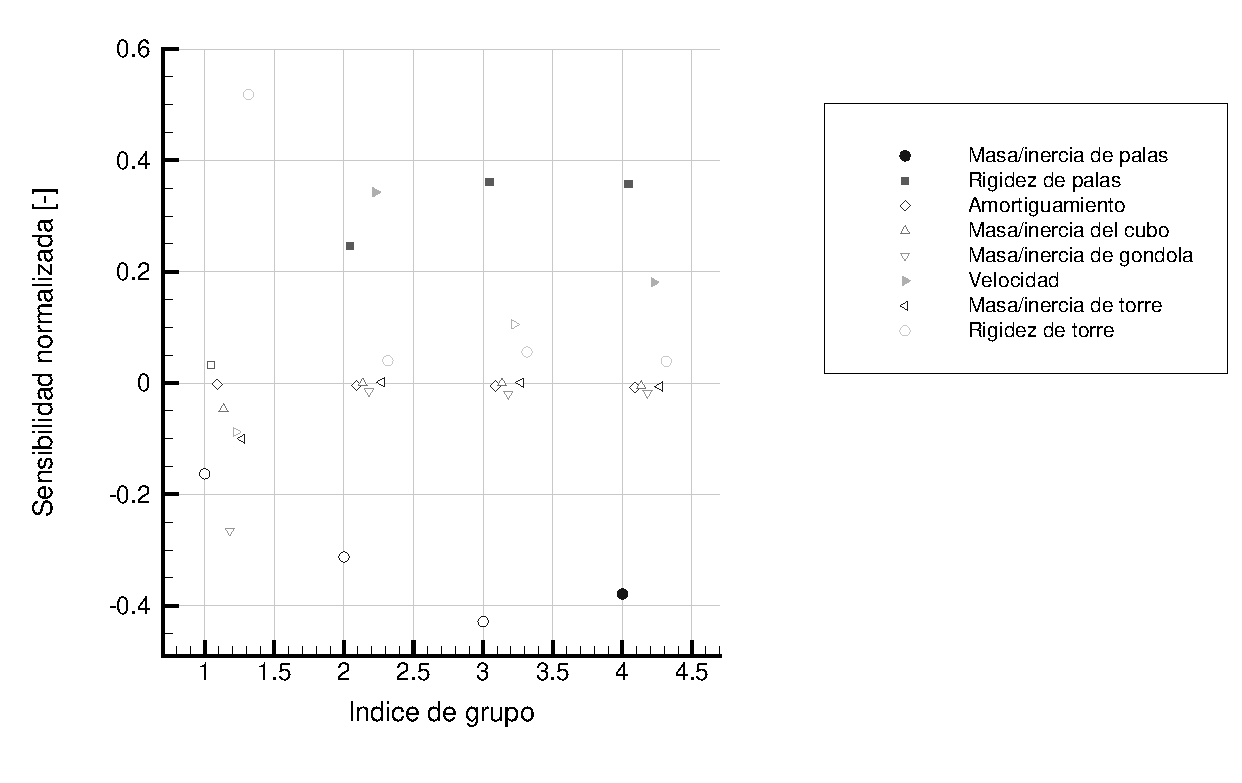
\includegraphics[width=.95\linewidth]{figures/tecplot/local_signos.pdf}
\caption{Secantes locales de frecuencia para el paso relativo 0.01. Los índices 1--4 corresponden a los grupos 1+2, 6+7, 8+9 y 10+11. Los marcadores llenos superan conjuntamente los controles de señal, seguimiento y estabilización; los vacíos conservan candidatos no resueltos y no deben interpretarse como efectos físicos aceptados. El pequeño desplazamiento horizontal separa parámetros dentro de cada grupo.}\label{fig:local-tecplot}
\end{figure}

\subsection{Respuesta temporal e interacciones}
Sean $R$ el mapa de traslaciones del suelo y $a_g$ su vector de aceleración. El benchmark sísmico conserva la proyección $-T^{\mathsf T}MRa_g$. Al escalar conjuntamente aceleración, velocidad y desplazamiento del suelo, los máximos de los cinco canales tienen sensibilidad unitaria, con desviaciones del orden de $6\times10^{-9}$. Es una verificación de linealidad del sistema congelado, no una validación sísmica de diseño.

Entre pasos de 0.0025 y 0.00125 s, la mayor diferencia relativa $L_2$ de desplazamiento fue $3.617\times10^{-4}$ y la mayor diferencia relativa de pico fue $2.378\times10^{-4}$. La tabla~\ref{tab:time} contiene los cuatro indicadores mecánicos aceptados con paso de 0.00125 s y $h=0.005$.

\begin{table}[htbp]
\centering\small
\caption{Sensibilidad de máximos absolutos en la ventana 0--1 s.}\label{tab:time}
\begin{tabular}{lllr}
\toprule
Factor & Nodo, componente global & Respuesta & $S_i$\\
\midrule
Densidad de palas & 128, $z$ & Aceleración absoluta & $+0.34213$\\
Rigidez de palas & 56, $z$ & Aceleración absoluta & $-1.03611$\\
Rigidez de palas & 128, $z$ & Desplazamiento relativo & $-0.16306$\\
Rigidez de palas & 128, $z$ & Aceleración absoluta & $-0.37885$\\
\bottomrule
\end{tabular}
\end{table}

La densidad modifica tanto los operadores de inercia/giro como la carga de base, por lo que no equivale a variar masa bajo fuerza externa constante. La rigidez modifica la transferencia dinámica y la precarga. Los signos de los máximos son observaciones de este registro corto; atribuirlos a resonancia de una rama requiere una descomposición adicional de la respuesta. No se establece una clasificación sísmica exhaustiva, pues solo se variaron estos dos factores mecánicos.

Las cuatro combinaciones a $\pm1\,\text{\char37}$ de densidad y rigidez producen estimaciones mixtas, pero ninguna estimación individual admisible supera el ruido. Además, se empleó un solo paso mixto. Se reportan como interacciones no resueltas y convergencia no verificada, sin afirmar existencia o ausencia de interacción física.

\section{Limitaciones y extensión propuesta}
Las conclusiones son locales y corresponden al benchmark heredado. Se mantienen las hipótesis existentes de colocalización y de inercia seccional, faltan calibración del tren y datos aerodinámicos, y no hay validación experimental. El espectro parcial a azimut fijo y la integración congelada no prueban estabilidad periódica ni simulan una historia de orientación del rotor.

Morris puede ser viable como segunda etapa de cribado sobre un dominio aprobado \cite{morris1991}. Con tres factores y cuarenta trayectorias requiere $40(3+1)=160$ evaluaciones básicas; el costo local medido sugiere aproximadamente veinte minutos de solución, antes de controles adicionales. Aún deben decidirse rangos y presupuesto. No se asignan distribuciones físicas ni se presenta el análisis de un parámetro por vez como sensibilidad global. Sobol no se justifica sin una medida conjunta de entrada. La propuesta exploratoria $[0.90,1.10]$ y un presupuesto de treinta minutos permanecen pendientes de decisión del autor.

Los datos crudos, fallos, opciones, estados y huellas se preservan. La corrección de postprocesamiento de la frontera espectral tiene procedencia separada y no cambia operadores o estados. Las figuras se entregan como PNG y PDF vectorial; esta sección autónoma requiere revisión antes de incorporarse al manuscrito.

